\documentclass[journal,10pt,twocolumn]{article}
\usepackage{graphicx}
\usepackage[margin=0.5in]{geometry}
\usepackage[cmex10]{amsmath}
\usepackage{array}
\usepackage{booktabs}
\usepackage{makecell}
\title{\textbf{Line Assignment}}
\author{Hari Venkateswarlu}
\date{September 2022}
\usepackage[framemethod=tikz]{mdframed}
\newcommand{\myvec}[1]{\ensuremath{\begin{pmatrix}#1\end{pmatrix}}}
\let\vec\mathbf
\newcommand{\mydet}[1]{\ensuremath{\begin{vmatrix}#1\end{vmatrix}}}
\providecommand{\mbf}{\mathbf}
\providecommand{\pr}[1]{\ensuremath{\Pr\left(#1\right)}}
\providecommand{\qfunc}[1]{\ensuremath{Q\left(#1\right)}}
\providecommand{\sbrak}[1]{\ensuremath{{}\left[#1\right]}}
\providecommand{\lsbrak}[1]{\ensuremath{{}\left[#1\right.}}
\providecommand{\rsbrak}[1]{\ensuremath{{}\left.#1\right]}}
\providecommand{\brak}[1]{\ensuremath{\left(#1\right)}}
\providecommand{\lbrak}[1]{\ensuremath{\left(#1\right.}}
\providecommand{\rbrak}[1]{\ensuremath{\left.#1\right)}}
\providecommand{\cbrak}[1]{\ensuremath{\left\{#1\right\}}}
\providecommand{\lcbrak}[1]{\ensuremath{\left\{#1\right.}}
\providecommand{\rcbrak}[1]{\ensuremath{\left.#1\right\}}}

\begin{document}

\maketitle
\paragraph{\textit{Problem Statement} - Find a point on the x-axis,which is equidistant from the points$\begin{pmatrix}
  7 \\
  6 \\
 \end{pmatrix}$ and $\begin{pmatrix}
  3 \\
  4 \\
 \end{pmatrix}$}
\begin{center}
    \label{tab:truthtable}
    \setlength{\arrayrulewidth}{0.2mm}
\setlength{\tabcolsep}{5pt}
\renewcommand{\arraystretch}{1.25}
    \begin{tabular}{|c|c|c|}
    \hline % <-- Alignments: 1st column left, 2nd middle and 3rd right, with vertical lines in between
      \large\textbf{Symbol} & \large\textbf{Co-ordinates} & \large\textbf{Description}\\
      \hline
       \large A & $\ \begin{pmatrix} 7\\ 6 \end{pmatrix}$ & co-ordinates of A \\
       \large B & $\ \begin{pmatrix} 3\\ 4 \end{pmatrix}$ & co-ordinates of B \\
	
	
      \hline
   \end{tabular}
 \end{center}\vspace{5mm}

\begin{figure}[h]
\centering
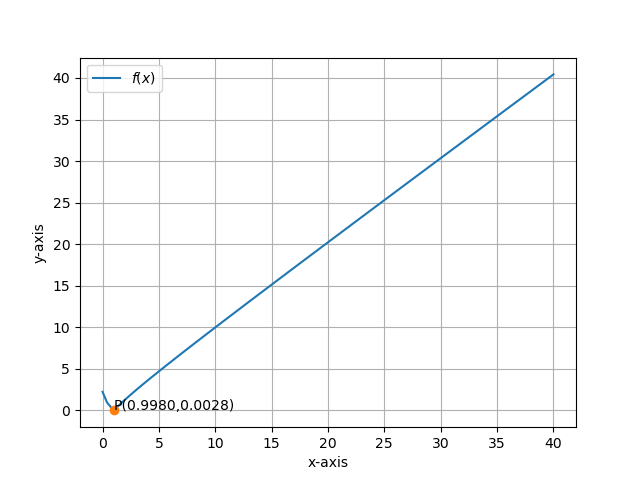
\includegraphics[width=1\columnwidth]{Figure1.png}

\label{fig}
\end{figure}

\section*{Solution}
1. Given points
A=$\begin{pmatrix}
  7 \\
  6 \\
 \end{pmatrix}$
 and B=$\begin{pmatrix}
  3 \\
  4 \\
 \end{pmatrix}$


\raggedright 2. If the point is lying on x-axis then y-axis will be zero i.e.. y=0

From the given information\\

\begin{align}
	\|\vec{(x-A)}\|^2 = \|\vec{(x-B)}\|^2
\end{align}  
    $\|\vec{(x-A)}\|^{\top} \vec{{(x-A)}} = \vec{(x-B)}\|^{\top} \vec{{(x-B)}}$\\          \vspace{2mm}
    $\|\vec{(x)}\|^2 - 2A^{\top}x + \|\vec{(A)}\|^2 = \|\vec{(x)}\|^2 - 2B^{\top}x + \|\vec{(B)}\|^2$\\ \vspace{2mm}    
    $\vec{2(A^{\top}-B^{\top})x} =  \|\vec{A}\|^2 - \|\vec{B}\|^2 $\\ \vspace{2mm}
    $\vec{(A^{\top}-B^{\top})x} = \frac{\|\vec{A}\|^2 - \|\vec{B}\|^2}{2}$\\ \vspace{2mm}
    $\vec{(A-B)^{\top}x} = \frac{\|\vec{A}\|^2 - \|\vec{B}\|^2}{2}$\\  \vspace{2mm}
\begin{align}
	\vec{e_2^{\top}x} = 0
\end{align}  
$\vec{(A-B)^{\top}x} = \frac{\|\vec{A}\|^2 - \|\vec{B}\|^2}{2}$\\ \vspace{2mm}
     $\myvec{0 & 1 \\ 4 & 2}x = $\myvec{0 \\ 30}\\ \vspace{2mm}
      $\myvec{0 & 1 & 0 \\ 4 & 2 & 30}$\\    \vspace{2mm}
      Divide by 2\\
      $\myvec{0 & 1 & 0 \\ 2 & 1 & 15}$\\    \vspace{2mm}
     $\myvec{2 & 1 & 15 \\ 0 & 1 & 0}
    \xleftarrow[]{R_2 \leftarrow R_1}$\\     \vspace{2mm}
    $\myvec{1 & \frac{1}{2} & \frac{15}{2} \\ 0 & 1 & 0}\xleftarrow[]{{R_1}=\frac{R_1}{2}}$\\            \vspace{2mm}
    $\myvec{1 & 0 & \frac{15}{2} \\ 0 & 1 & 0}\xleftarrow[]{{R_1}={R_1}-\frac{R_2}{2}}$\\             \vspace{2mm}
    $\myvec{1 & 0 & 7.5 \\ 0 & 1 & 0}$\\        \vspace{2mm}
on solving we get x = 7.5\\
\vspace{2mm}
  x=$\begin{pmatrix}
  7.5 \\
  0 \\
 \end{pmatrix}$               			
\end{document}
